\documentclass[tikz,border=10pt]{standalone}
\usetikzlibrary{calc,intersections}
\begin{document}
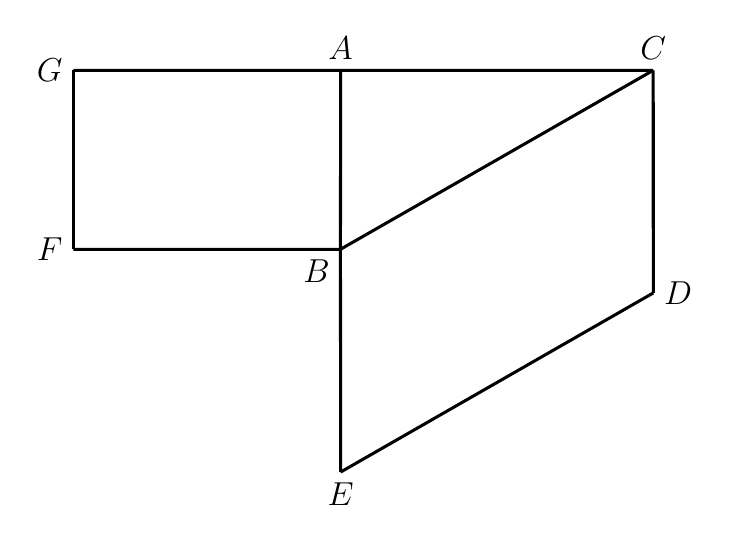
\begin{tikzpicture}[line join=round, line width=1.1pt, font=\fontsize{12}{14.4}\selectfont]
\coordinate (A) at (-0.144,2.561);
\coordinate (B) at (-0.146,0.289);
\coordinate (C) at (3.826,2.562);
\coordinate (D) at (3.827,-0.265);
\coordinate (F) at (-3.539,0.288);
\coordinate (G) at (-3.539,2.561);




\coordinate (E) at (-0.144,-2.540);


\path[name path=GC] (G) -- (A) -- (C);
\draw[name path=GC] (G) -- (A) -- (C);

\path[name path=FG] (F) -- (G);
\draw[name path=FG] (F) -- (G);

\path[name path=FB] (F) -- (B);
\draw[name path=FB] (F) -- (B);

\path[name path=ABE] (A) -- (B) -- (E);
\draw[name path=ABE] (A) -- (B) -- (E);

\path[name path=CB] (C) -- (B);
\draw[name path=CB] (C) -- (B);

\path[name path=CD] (C) -- (D);
\draw[name path=CD] (C) -- (D);

\path[name path=DE] (D) -- (E);
\draw[name path=DE] (D) -- (E);


\node[above] at (A) {$A$};
\node[above] at (C) {$C$};
\node[left] at (G) {$G$};
\node[left] at (F) {$F$};
\node[below left] at (B) {$B$};
\node[right] at (D) {$D$};
\node[below] at (E) {$E$};
\end{tikzpicture}
\end{document}